Active hand prostheses (AHPs) are hand prostheses which can be
voluntarily actuated, to some degree, by the patient who is wearing
them. The ideal AHP is cheap, visually appealing, lightweight,
dexterous and, lastly, easily and naturally controlled. Moreover, it
provides sensorial feedback to the amputee. At the time of writing,
however, the state-of-the-art of AHPs is far from this. The best
commercially available AHPs are probably Otto Bock's SensorHand and
Touch Bionics's i-Limb, both of which have a very limited number of
degrees of freedom and are hardly able to replicate the human hand's
movements and postures.

Nevertheless, one can see a definite move forward as far as the
mechatronics is concerned --- a drive which mainly comes from
miniaturised electronics and humanoid robotics; examples of this are,
e.g., the DLR prosthetic hand (\cite{Hua2006}---see Figure
\ref{fig:DLRHandII}) and the the CyberHand \cite{cyberhand}. More
degrees of freedom and human-like features are seen at the horizon;
the i-Limbs, for instance, has five moving fingers and a passively
opposable thumb, although it is so far controllable only in a few
ways.

\begin{figure}
  \begin{tabular}{cc}
    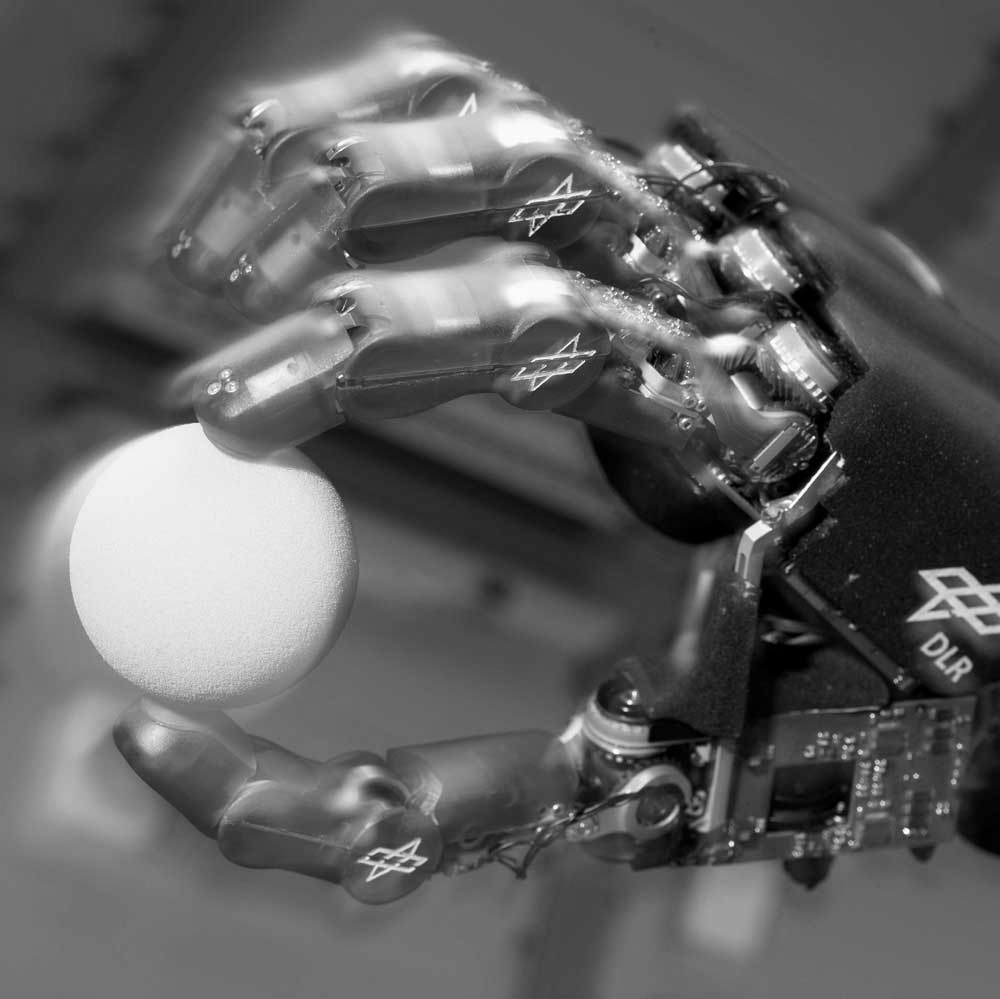
\includegraphics[height=0.12\textheight]{figs/DLRHand-Ball-comp.jpg} &
    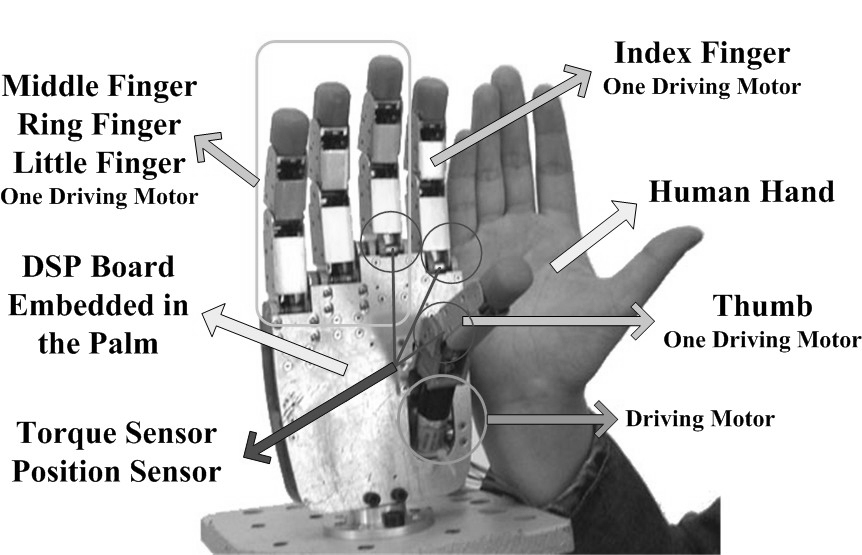
\includegraphics[height=0.12\textheight]{figs/DLR-Prothese.jpg}
  \end{tabular}
  \caption{(left) The DLR Hand II. (right) The DLR prosthetic hand.}
  \label{fig:DLRHandII}
\end{figure}

Still, it is unclear how to effectively \emph{control} an AHP. So far,
the best, cheapest and simplest control strategy has been that
provided by surface electromyography (EMG); but usually, at most, one
or two electrodes are used, to detect strictly independent muscle
activation potentials. These potentials control, at best, one degree
of freedom of the prosthesis and a ``switch'' to change from, e.g.,
opening and closing the hand to flecting/extending the elbow. On the
other hand, operating well an AHP would require a fine control,
possibly down to the level of the single fingers, all the more reason
now that more dexterous and flexible AHPs are being available on the
market.

In the ideal scenario, presented with a certain task such as turning a
door handle or grabbing a car key, the patient should be able to
enforce the correct grasping type; this involves the activation of
some joints only, and in particular positions. Secondly, the amount of
force involved in the grasp must be controlled, so that it is possible
to grab, e.g., both a hammer without letting it slip and an egg
without breaking it.

This paper is an initial attempt at solving this problem. Our aim, in
the long run, is that of enabling a patient to optimally and naturally
control an AHP with many degrees of freedom and the possibility of
modulating the involved force. To this end, provided that the patient
still has enough muscular activity in the stump, we believe the best
way is the use of forearm surface EMG. This technique is (rather)
cheap and involves no surgery; and, we believe, it can be used to
detect what the patient wants the prosthesis to do.

In our experiment, over two days, we have gathered forearm surface EMG
data from a healthy subject gripping in four distinct ways a force
sensor; we have then trained three different machine learning systems
to guess

\begin{enumerate}

  \item what kind of grasp the subject was doing, e.g., thumb and
    index finger, thumb and middle finger, thumb and ring finger or
    thumb and all other fingers; and

  \item how much force the subject was exerting, in order to
    understand whether the grasp was, e.g., a power grasp or rather a
    precision grip. Surprisingly, as far as we know, nobody has ever
    attempted so far to solve this problem, although it is well-known
    that the EMG is related to the force a muscle is exerting.

\end{enumerate}

The three approaches we have experimented with are:
(a) a simple feed-forward neural network with one hidden layer,
(b) a Support Vector Machine with radial basis function kernel
\cite{BGV92}, and (c) Locally Weighted Projection Regression
\cite{lwpr}. These approaches were chosen mainly because SVMs already
have shown good performance when trained to classify isometric hand
postures (see, e.g., \cite{smagt}). Notice that the problem here is
rather more complicated by the fact that the hand is obviously moving
while grasping. For comparison, we decided to check whether neural
networks could outperform SVMs (neural networks are probably the most
popular machine learning method nowadays). For further comparison, we
employed LWPR as a more heuristic approach, designed since the
beginning to work in an online setting.

Our analysis consists of a preliminary phase in which several models
have been built in a batch fashion, in order to understand how to deal
with the non-stationarity of EMG. The most interesting challenge has
been how to filter out unwanted data, at the same time keeping a high
overall accuracy, both in classification and regression. Later on,
based upon the results obtained in the preliminary phase, we have
developed a simple but effective procedure for selecting a subset of
the samples on-the-fly, called \emph{Online Uniformisation} (OU).

OU is based upon the simple idea of keeping a minimum inter-sample
Euclidean distance, in order to uniformly sample the input space. The
selected samples are then used to periodically re-train the system,
and check that it has adapted to the new data. The training sets thus
obtained are remarkably small and thus usable on-line, and they offer
an excellent trade-off between size and accuracy. In particular, as a
certain parameter is increased, the size of the uniform training sets
decreases polynomially, while the error rate increases only
linearly; therefore one can obtain much smaller training sets (which
means faster or more adaptive machines) by accepting an error rate
which is only linearly worse.

This behaviour appears in both problems highlighted above (the former
involving classification, the latter regression), and for all the
approaches tested. Our numerical results indicate that, in such a
scenario, the type of grasp can be reconstructed with an average
accuracy of $89.67\% \pm 1.53\%$, and the applied force can be
predicted with an average percentage error of $7.89\% \pm 0.09\%$,
meaning $4.5$N over a range of about $57$N.

The paper is structured as follows: after a brief review of relevant
literature, we describe in detail the experiment and the methods used
to tackle it (Section \ref{sec:m&ms}); then we show and comment on the
experimental results, both the preliminary phase and the online
experiments (Section \ref{sec:exp}); lastly, discussion and
conclusions are presented.
